\documentclass[conference]{IEEEtran}
\IEEEoverridecommandlockouts
% The preceding line is only needed to identify funding in the first footnote. If that is unneeded, please comment it out.
\usepackage{cite}
\usepackage{amsmath,amssymb,amsfonts}
\usepackage{algorithmic}
\usepackage{graphicx}
\usepackage{textcomp}
\usepackage{listings}
\usepackage{xcolor}
\def\BibTeX{{\rm B\kern-.05em{\sc i\kern-.025em b}\kern-.08em
    T\kern-.1667em\lower.7ex\hbox{E}\kern-.125emX}}
\begin{document}

\title{AI Compute System Lab3 Report\\
}

\author{\IEEEauthorblockN{Guanghui Hu} 2024234318}

\maketitle

\lstset{
  language=Verilog,              % 设置语言为 Verilog
  basicstyle=\ttfamily\small,    % 基本字体样式
  keywordstyle=\color{blue},     % 关键字颜色
  stringstyle=\color{red},       % 字符串颜色
  commentstyle=\color{gray},     % 透明灰色注释
  breaklines=true,               % 自动换行
  tabsize=2,                     % Tab 宽度
  captionpos=b,                  % 标题位置(b 表示底部,t 表示顶部)
}

\section{Introduction}

The lab required the construction of a simple hardware system.
It is capable of implementing in-memory data format conversions,
as well as an operator to accelerate matrix multiplication.
The top design is described in \verb|vsrc/sim/top.v|.
The top design mainly consists of three main modules:

\begin{itemize}
    \item im2col: Converting ordinary matrix into easily convoluted forms.
    \item systolic array: Implement acceleration of matrix multiplication.
    \item memory: save input matrix, weight matrix and outputs matrix.
\end{itemize}

\verb|im2col| module connects to memory by address and data bus.
It should load input matrix from memory and store outputs matrix to memory.
The lab guide mentions that "For the input and weight tensors stored in memory, they are both stored in NHWC format.
The two-dimensional matrix X obtained after Im2Col is stored in \verb|X_buffer| in column-major order.
The weight matrix W and the GEMM output matrix ,
are stored in \verb|W_buffer| and \verb|Y| in row-major order, respectively".
This means that \verb|m2col| module needs to load and store to a different matrix data format.

\verb|systolic array| module get input matrix and weight matrix in the form of a systolic array.
This means it aquires one column or one row of input matrix or weight matrix in one cycle.
At the completion of the data transfer, it needs to compute the multiplication of the two matrices.
and output the result in one cycle.

\verb|memory| is a variable in top module.
It provides data load and store operations to other modules,
like \verb|im2col| and \verb|systolic| array.
Note that this is an ideal storage model,
requiring only one clock cycle to read or write data.
Therefore, there is no memory protocols, such as AXI4, CHI.
Only address, data, read write enable, three signals is to complete the access operation.
In particular, when he provides data to \verb|systolic array|,
It load a column of input matrix and row of weight matrix at one cycle,
and send data to \verb|systolic array|.
Data is held for just one clock cycle.
Hence, if \verb|systolic array| is can not to process all the input data in one cycle,
it needs to save the input data in register by itself, otherwise it will result data missing.

\section{Implementation}

This chapter describes the implementation of the im2col and systolic array in detail,
which is mentioned in the previous chapter.

\subsection{im2col}
This module performs the matrix format conversion.
The code implementation is located in \verb|vsrc/src/im2col.v|.
All input signals are shown in the \ref{tab:im2col_if}.
Note that the output \verb|done| indicates the completion of the conversion.
The signal must be set after all memory access operations have been completed,
otherwise there is write-after-read hazard in memory.

\begin{table}[ht]
    \caption{im2col's interface}
    \centering
    \begin{tabular}{|l|l|l|l|}
        \hline
        \textbf{name} & \textbf{type} & \textbf{width} & \textbf{description}    \\ \hline
        clk           & input         & 1              & clock signal            \\ \hline
        rst\_n        & input         & 1              & reset signal            \\ \hline
        data\_rd      & input         & DATA\_WIDTH    & the value read from mem \\ \hline
        data\_wr      & output        & DATA\_WIDTH    & the value write to mem  \\ \hline
        addr\_rd      & output        & ADDR\_WIDTH    & memory read address     \\ \hline
        addr\_wr      & output        & ADDR\_WIDTH    & memory write address    \\ \hline
        done          & output        & 1              & operation done signal   \\ \hline
        mem\_wr\_en   & output        & 1              & memory write enable     \\ \hline
    \end{tabular}
    \label{tab:im2col_if}
\end{table}

Additionally, all parameters are shown in the \ref{tab:im2col_pa}.
The parameter \verb|FILTER_SIZE| will generate \verb|PAD_SIZE|,
which define the input image need to zero-padding or not.
whereas for 1x1 kernels, padding is not needed.

\begin{table}[ht]
    \caption{im2col's parameters description}
    \centering
    \begin{tabular}{|l|l|}
        \hline
        \textbf{name} & \textbf{description}       \\ \hline
        IMG\_C        & image channel              \\ \hline
        IMG\_W        & image width                \\ \hline
        IMG\_H        & image height               \\ \hline
        DATA\_WIDTH   & data width                 \\ \hline
        ADDR\_WIDTH   & address width              \\ \hline
        FILTER\_SIZE  & size of convolution kernel \\ \hline
        IMG\_BASE     & image base address         \\ \hline
        IM2COL\_BASE  & im2col base address        \\ \hline
    \end{tabular}
    \label{tab:im2col_pa}
\end{table}

The state machine design is used to implement the matrix format transformations.
there are three state: \verb|LOAD|, \verb|STORE| and \verb|DONE|.
When the reset signal is set, state is assigned to \verb|LOAD|,
if the current state is \verb|LOAD|, the next state is \verb|STORE|,
until the last element is stored to memory, the state is set \verb|DONE|.
In order to keep track of which element is currently being processed,
register counters are necessary.
In this design, an order that is consistent with human reading habits is used when processing:
based on the output matrix, from left to right, from top to bottom.
The output matrix element number is
\[
  (H_{img} \times W_{img} , FILTER\ SIZE^2 \times C_{img})
\]
Therefore, there are five register counters:
\verb|h|, \verb|w|, \verb|c|, \verb|row| and \verb|col|.
Obviously, \verb|h| and \verb|w| represent the current location of the convolution kernel.
\verb|c| correspond to IMG\_C in \ref{tab:im2col_pa}.
\verb|row| and \verb|col| are filter's row and column.
They both count from 0 to FILTE\_SIZE.
All counters register in im2col is assign to zero when reset.
And they are nested and incremental as shown in \ref{code:nested_cnt}

\begin{lstlisting}[
    caption={Nested Counters Implementation},
    label={code:nested_cnt}
]
/* nested counters */
reg [ADDR_WIDTH-1:0] counters [0:4];
wire [ADDR_WIDTH-1:0] cnt_next [0:4];
wire is_max [0:4];
/* verilator lint_off UNOPTFLAT */
wire wrap_next [0:4];

generate
  for (genvar i=1; i<5; i=i+1) begin
    always @(posedge clk) begin
      if (!rst_n || done) begin
        counters[i] <= 0;
      end
      else begin
        if (wrap_next[i-1] && tick) begin
            counters[i] <= cnt_next[i];
        end
      end
    end
    assign wrap_next[i] = 
        wrap_next[i-1] && is_max[i];
  end
endgenerate
\end{lstlisting}
The load address, store address and is padding or not can be calculated from these five register counters.
The essence of im2col module is that it constantly load and store based on the current state and the counters.
When all counters meet his maximum value, signal done is set.

\subsection{systolic array}

This module calculate two input matrices multiplication and save result in registers.
The code implementation is located in \verb|vsrc/src/systolic_array.v|.
All input signals are shown in the \ref{tab:syst_if}.
And all parameters are shown in the \ref{tab:syst_pa}.

\begin{table}[ht]
  \caption{systolic array's interface}
  \centering
  \begin{tabular}{|l|l|l|l|}
    \hline
    \textbf{name} & \textbf{type} & \textbf{width}                & \textbf{description}  \\ \hline
    clk           & input         & 1                             & clock signal          \\ \hline
    rst\_n        & input         & 1                             & reset signal          \\ \hline
    X             & input         & DATA\_WIDTH$\times$M          & inputs on X side      \\ \hline
    W             & input         & DATA\_WIDTH$\times$K          & weights on W side     \\ \hline
    Y             & output        & DATA\_WIDTH$\times$M$\times$K & outputs in all PEs    \\ \hline
    done          & output        & 1                             & operation done signal \\ \hline
  \end{tabular}
  \label{tab:ports_description}
  \label{tab:syst_if}
\end{table}

\begin{table}[ht]
  \caption{im2col's parameters description}
  \centering
  \begin{tabular}{|l|l|}
    \hline
    \textbf{name} & \textbf{description}  \\ \hline
    M             & number of X's rows    \\ \hline
    N             & number of X's columns \\ \hline
    K             & number of W's rows    \\ \hline
    DATA\_WIDTH   & data width            \\ \hline
  \end{tabular}
  \label{tab:syst_pa}
\end{table}

Note that the output \verb|done| indicates the completion of the multiplication.
The signal must be set after all Y's elements have been completed.
Besides, X and W value are only be kept by one cycle.
but systolic array can not process one one column or one row in one cycle,
It delay one cycle for second element and delay two cycle for third element.
, until the M-th element will be delayed M-1 cycle.
This less repetitive logic is difficult to write by hand in Verilog
and can be generated using the \verb|generate| statement as shown in the \ref{code:delays}.
Module \verb|Repeater| is instantiated to delay the input data.
The parameter \verb|cycleNR| specifies the number of cycle
for which the input signal needs to be delayed.

\begin{lstlisting}[
    caption={Inputs Delay Implementation},
    label={code:delays}
]
generate
  for (genvar m=0; m<M; m=m+1) begin
    wire [DATA_WIDTH-1:0] data_in  = X[(m+1)*DATA_WIDTH-1:m*DATA_WIDTH];
    wire [DATA_WIDTH-1:0] data_out;
    assign x_in[m][0] = data_out;
    Repeater #(
      .cycleNR(m),
      .DATA_WIDTH(DATA_WIDTH)
    ) rep_x (
      .clk(clk),
      .rst_n(rst_n),
      .data_in(data_in),
      .data_out(data_out)
    );
  end
endgenerate
\end{lstlisting}

The other major component of systolic array is the PE array.
Each PE passes the input data and weights to neighboring PEs.
This is also implemented by \verb|generate| block in \ref{code:pes}.
Variables \verb|x_in| and \verb|w_in| is declared with type \verb|wire|.
They are both two-dimensional array,
representing the connection wires bewteen PEs.
Indexing an array with a \verb|genvar| variables make it easy
to get the connecting wire between PEs.

\begin{lstlisting}[
    caption={PE Array Implementation},
    label={code:pes}
]
wire [DATA_WIDTH-1:0] x_in [M-1:0][K:0];
wire [DATA_WIDTH-1:0] w_in [M:0][K-1:0];
generate
  for (genvar m = 0; m < M; m = m + 1) begin
    for (genvar k = 0; k < K; k = k + 1) begin
      wire [DATA_WIDTH-1:0] y_out;
      pe#(
        .DATA_WIDTH(DATA_WIDTH)
      ) pe (
        .clk(clk),
        .rst(rst_n),
        .x_in   (x_in[m  ][k  ]),
        .w_in   (w_in[m  ][k  ]),
        .x_out  (x_in[m  ][k+1]),
        .w_out  (w_in[m+1][k  ]),
        .y_out  (y_out)
      );
      assign Y[m*K*DATA_WIDTH+(k+1)*DATA_WIDTH-1:m*K*DATA_WIDTH+k*DATA_WIDTH] = y_out;
    end
  end
endgenerate
\end{lstlisting}

Single PE unit implementation is simple,
only need to set up some registers for calculating and saving data, as shown in the \ref{code:pe}.

\begin{lstlisting}[
    caption={PE Implementation},
    label={code:pe}
]
always @(posedge clk) begin
  if (!rst) begin
    y_out <= 0;
    x_out <= 0;
    w_out <= 0;
  end
  else begin
    y_out <= y_out + (x_in * w_in);
    x_out <= x_in;
    w_out <= w_in;
  end
end
\end{lstlisting}

On the basis of the above design,
the implementation \verb|systolic array| module is very simple.
Only need to add a register counter to count the number of clock cycles
that need to be calculated.
For input matrix, it takes $M - 1$ clock cycles for the data in the first column to enter the module.
And there are $N$ columns data, taking $N$ clock cycle.
Finally, the last column data need to reaches the last element of the array,
which takes $K$ cycles.
Totally $M + N + K - 1$ cycles after reset, signal \verb|done| can be set.

\section{Conclusion}

The above design can pass the automated simulation test.
Command \verb|make test| will compiled design by verilator,
generating elf file, runing to dump memory, comparing data by python scripts.
Figure \ref{fig:pass} shows the output of make command.
It is clear that this design pass the test.

\begin{figure}[ht!]
  \centering
  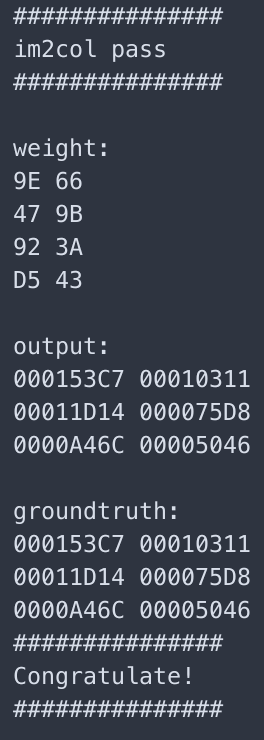
\includegraphics[width=0.15  \textwidth]{pass.png}
  \caption{outputs of make test}
  \label{fig:pass}
\end{figure}

In lab3, a system to accelerate convolutional is implemented by verilog language.
It transforming convolution operations into General Matrix Multiplications(GEMM) by module \verb|Im2Col|.
And compute matrices multiplication by \verb|Systolic Array|.
Finite state machines, generate statements, nested counters, repeaters, etc.
are used in the design of the system.
They simplify the code of the design while ensuring its correctness.
Finally, the design is verified to be able to achieve GEMM acceleration for convolutional.


\end{document}
